\chapter{Hardware}

\missingfigure{Photograph of final board revision} 

\section{Board Overview}
The principal aim of the design was to develop an energy and reasonably cost-efficient wireless sensing platform, with easy expandability so as to support arbitrary sensor attachments. This section discusses the design and implementation of the board, along with the rationale behind certain hardware choices.

The designed sensor platform is a small, credit-card sized board. Temperature, humidity, and ambient light-levels are measured on-board, while the remaining micro-controller general purpose input-output (GPIO) is broken out to a standard 0.1" pitch header. The board is based on the Texas Instruments CC3200 system-on-a-chip (SOC), containing an ARM-M4 MCU and an 802.11 WiFi radio.

\section{Microcontroller}

\begin{table}[h]
\caption{Microcontroller comparison}
\label{uc-comparison}
\resizebox{\textwidth}{!}{%
\begin{tabular}{@{}l|llll@{}}
 & Texas Instruments CC3200 & Freescale Kinetis KW2x & ST Microelectronics STM32W108CB & Atmel ATSAMR21E17A \\ \midrule
Flash Memory & External & Up to 512 KB & Up to 256 KB & Up to 256 KB \\
RAM & Up to 256 kB & Up to 64 KB & Up to 16 KB & Up to 32 KB \\
Processor & ARM Cortex-M4 & ARM Cortex-M4 & ARM Cortex-M3 & ARM Cortex-M0+ \\
Clock frequency & 80 MHz & 50 MHz & 24 MHz & 48 MHz \\
Operating Current ex. Transceiver & 15.3 mA @ 3.6V & 17 mA @ 3.0 V & Not specified & Not specified \\
ADC & 12 bit SAR & 16 bit SAR & 12-bit Sigma Delta & 12-bit SAR \\
In-application programming & Yes & Yes & Yes & Yes \\
Operating Voltage & 2.1V - 3.6V & 1.8V - 3.6V & 2.1V - 3.6V & 1.8V - 3.6V \\
General purpose I/O pins & 27 & 24 & 24 & 28
\end{tabular}
}
\end{table}

The Texas Instruments CC3200 was chosen after evaluating several different chips from Freecale, Atmel, and other manufacturers. A sample comparison is presented in table \ref{uc-comparison}. Important characteristics for a microcontroller were: 1) power consumption, 2) memory size, 3) easy of programmability, and 4) transceiver integration. The CC3200 is neither very low power nor is it very inexpensive due to requiring an external flash memory module. However, it has several advantages as a chipset for a residential sensing platform. First, it supports 802.11b/g/n, which is ubiquitous in residential buildings. Given the typical 4-5 node scale of an ecoMOD deployment, not having to purchase an inter-networking gateway more than makes up for the slightly higher cost of the chip, which is around \$11 in quantity from DigiKey. Second, it is based on the Arm Cortex-M4 microcontroller, which means it can be programmed with open-source (i.e., free) toolchains, and has a floating-point coprocessor for digital signal processing. Finally, the CC3200 is a hybrid package, with an integrated balun and matching network. Any single-ended 50 Ohm antenna can be connected and it will theoretically just work, which is the exception, and not the rule.

\begin{figure}[h]
\centering
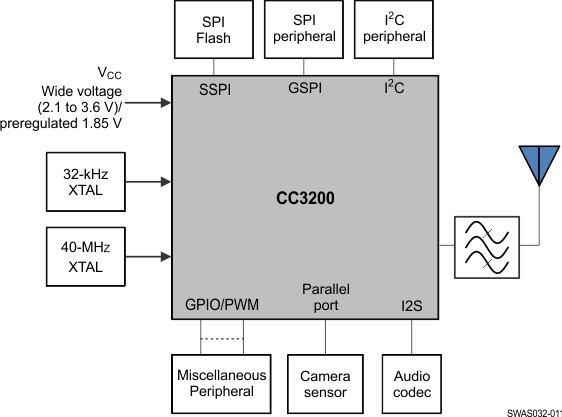
\includegraphics[width=0.5\linewidth]{images/cc3200-block}
\caption[CC3200 Block Diagram]{Block diagram of CC3200 functionality\cite{2015}}
\label{fig:cc3200-block}
\end{figure}

\begin{table}[h]
\caption{CC3200 figures of merit}
\label{CC3200-fom}
\begin{tabular}{@{}l|l@{}}
\toprule
Voltage Supply                  & 2.1V - 3.6V \\
Clock Frequency                 & 80 MHz      \\
Maximum Current Draw @ 14.5 dBm & 229 mA      \\
Sleep, Radio Idle Listen        & 695 uA      \\
Sleep, All Systems              & 129 uA      \\
Hibernate                       & 4 uA        \\
RAM                             & 128 KB      \\
Flash Storage                   &             \\ \bottomrule
\end{tabular}
\end{table}

\section{Sensors}

An environmental monitoring platform is useless without some way of measuring the environment. Although the design includes a 0.1" header for expandability, light, temperature, and humidity sensing was included on board. Where possible, I2C compatible sensors were chosen for ease of integration and lowered parts count. The sensor characteristics are summarized in Table \ref{sensor-specs}. The bottom two entries in the table consist of external sensors that were connected to the microcontroller's ADC. 

\begin{table}[h]
\caption{Sensor specifications}
\label{sensor-specs}
\resizebox{\textwidth}{!}{%
\begin{tabular}{@{}l|llllll@{}}
 & Active Power Use & Operating Voltage & Sense range & Accuracy & Interface & Product No. \\ \midrule
Temperature & \multirow{2}{*}{27 uW combined} & 1.5V -3.6V &  & 0.3degC & I2C & HTU21D(F) \\
Humidity &  & 1.5V-3.6V & 0-100\% RH & 2\% RH & I2C & HTU21D(F) \\
Light & 0.75 mW & 2.7V-3.6V & Up to 40 kLux & Wavelength dependent & I2C & TSL2561 \\
Force & passive resistive & N/A & up to 1000 lbs & 3\% of max range & Analog & ZFLEXA201 \\
Soil Moisture & 24 mW & 3.5V - 20V & 0-50\% water by volume & 2\% & Analog & VH400
\end{tabular}
}
\end{table}

\subsection{Light}

The light sensor is the TSL2561. The response curve approximates the sensitivity of the human eye. Light levels are important in measuring solar insolation, which affects building heating and cooling schedules. This particular sensor contains two photodiodes on board - one more responsive to infra-red, and the other with an even full-spectrum frequency response curve. It is pre-calibrated from the manufacturer, and utilizes an SMBus/I2C interface.

\subsection{Humidity and Temperature}

The board mounts an integrated relative humidity and temperature sensor from Taos: the TSL2561. Accurate measurement of relative humidity is highly dependent on the atmospheric temperature. As a result, most instrumentation-grade humidity sensors come with a temperature sensor for free. The sensor is based on sensing changes in capacitance, and comes pre-calibrated from the factory. Humidity and temperature must be known in order to determine heating and cooling energy expenditures.

\begin{figure}[h]
\centering
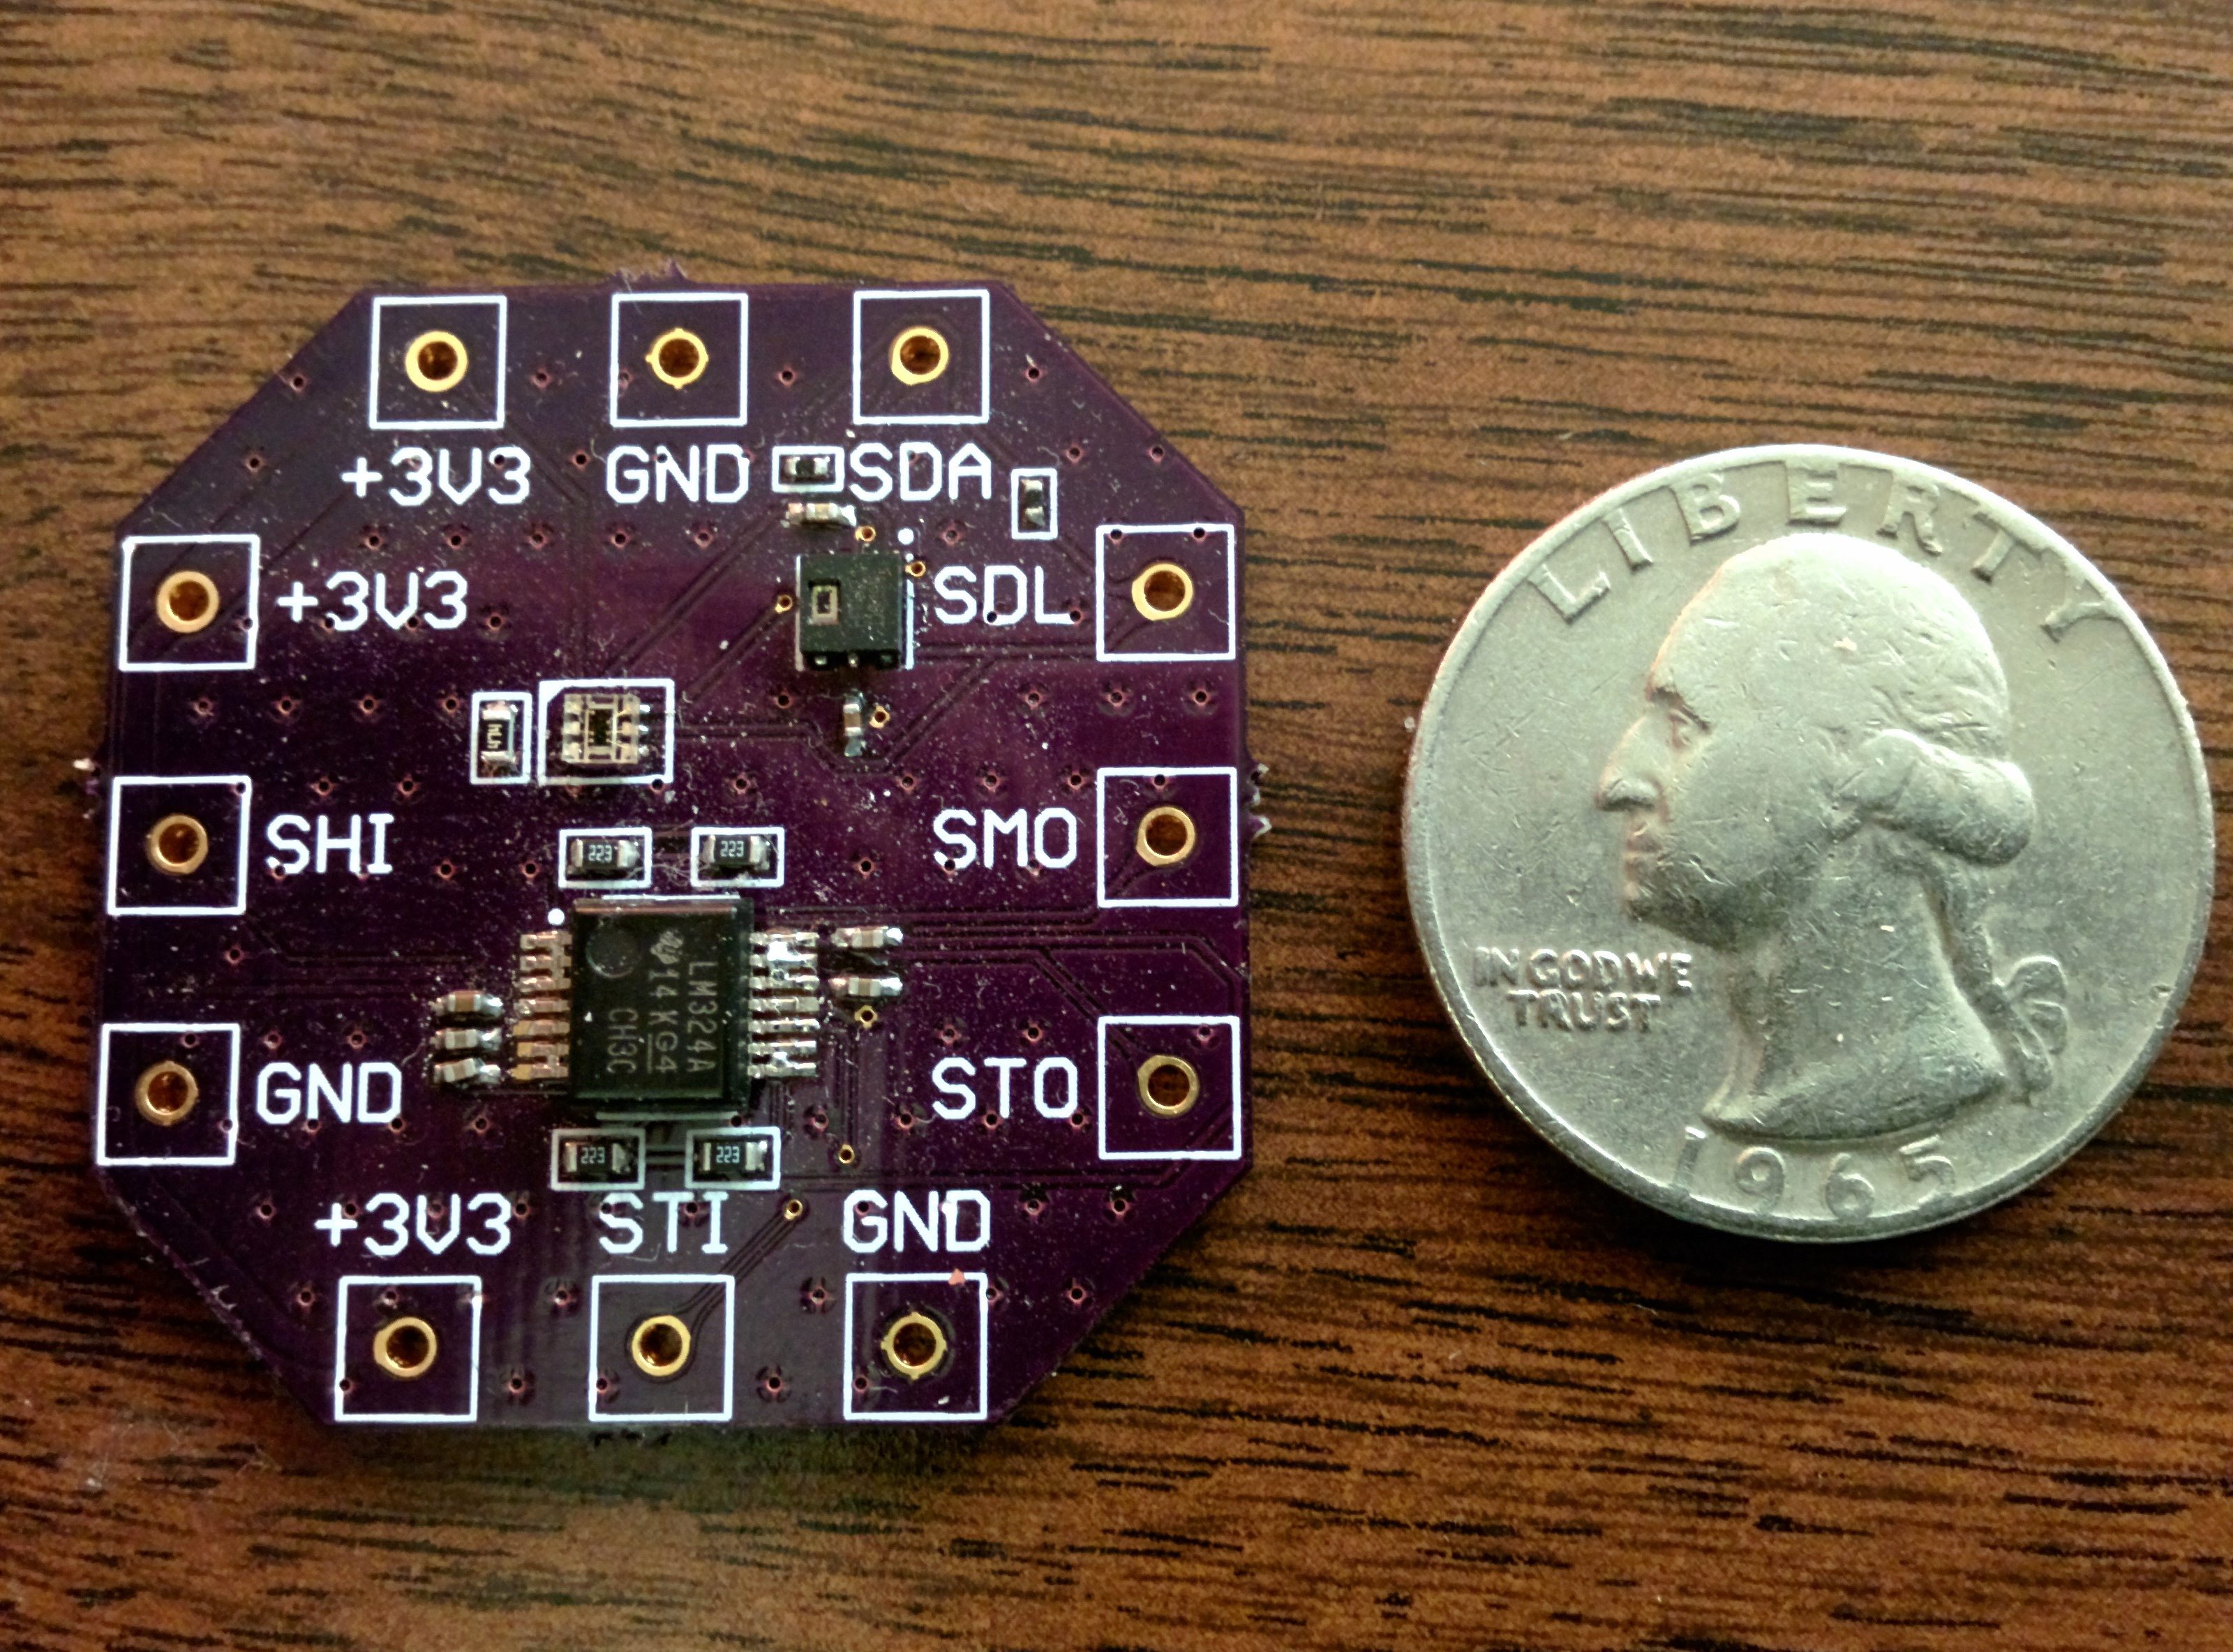
\includegraphics[width=0.3\linewidth]{images/sbrk-proto}
\caption[Development breakout]{Breakout prototype board containing quad op-amp for soil moisture voltage conditioning, and humidity, temperature, and light sensor I2C lines}
\label{fig:sbrk-proto}
\end{figure}

\subsection{Other}
\subsubsection{Force Sensing}
A piezoelectric resistive force sensor from Flexiforce was tested. Force and pressure measurements are useful for measuring foot traffic. 

\begin{figure}[h]
\centering
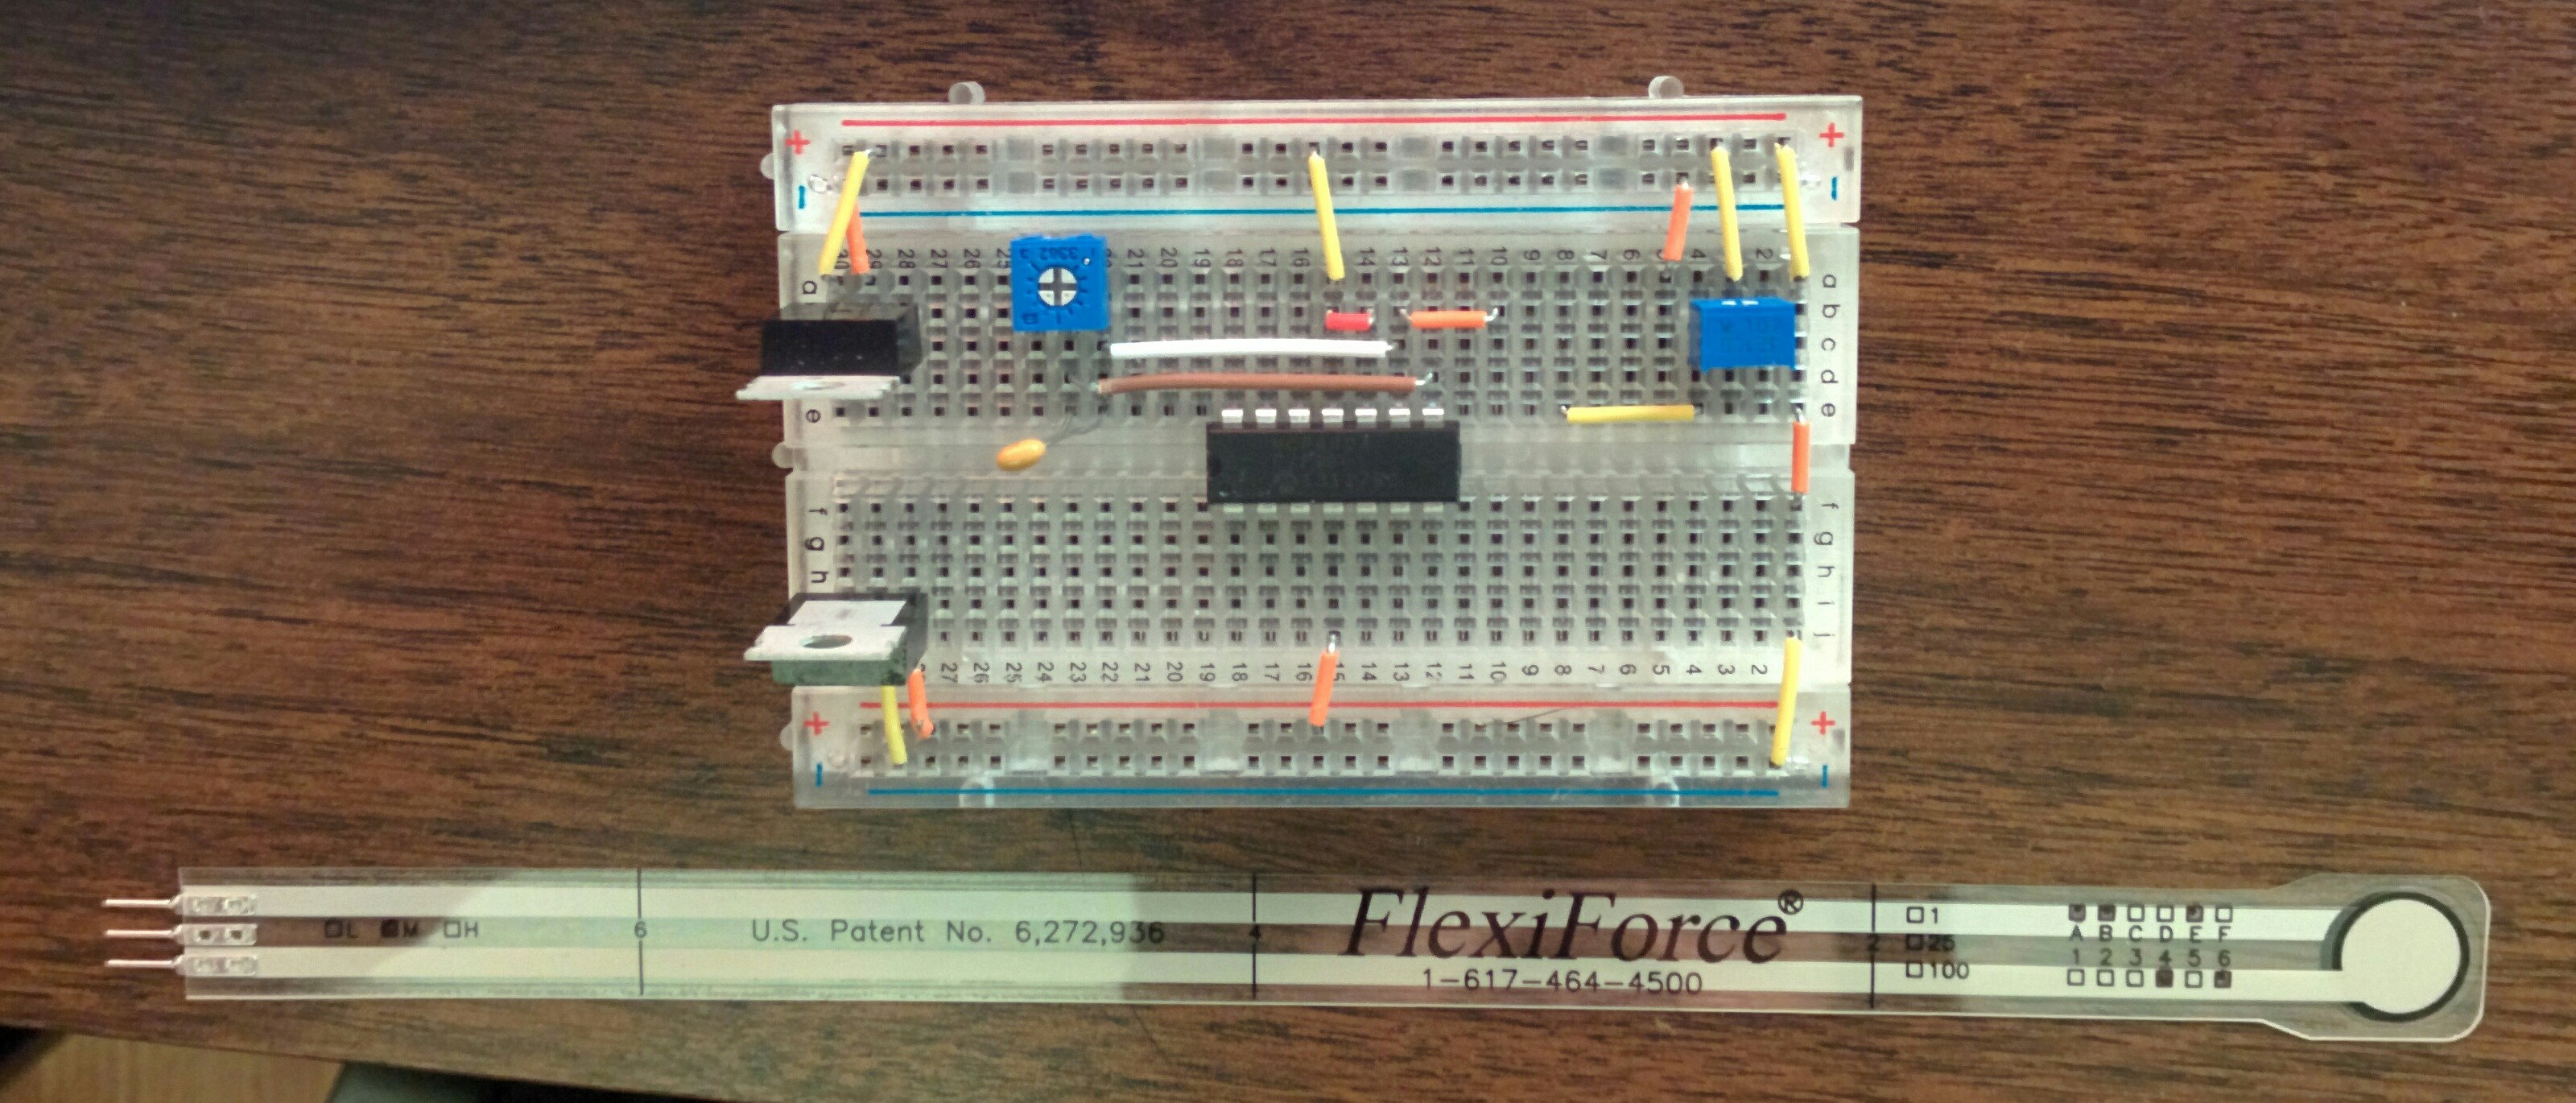
\includegraphics[width=0.33\linewidth]{images/force-proto}
\caption[Force sensor prototype]{Force sensor prototype circuit with an analog low-pass filter and adjustable gain}
\label{fig:force-proto}
\end{figure}

\subsubsection{Soil Moisture Sensing}
A capacitive soil moisture sensor from Vegetronix was also tested. Soil moisture was an important environmental measure needed for ecoMOD 4, which had a ground source heat pump. The greater the soil moisture, the more thermal capacity the heat pump has to draw on. The sensor has an output voltage range of 0 to 3V. As the CC3200 ADC inputs can only tolerate a maximum voltage of 1.46V; the sensor output voltage must be divided by two for full range operation. The same circuit used for the force sensor prototype can be used to interface the soil moisture sensor, with adjustments to the potentiometer resistance ratios.

\section{Radio}

IEEE 802.11 (WiFi) has traditionally been used to provide high-speed, moderate range data transfer. Typical systems utilizing it have been fast but not energy-efficient, which has led to the perception of it being unsuitable for use in long-lifetime battery-powered devices. However, this is not from any inherent inefficiency in the protocol. In fact, the raw energy per bit transmitted is competitive with other protocols such as 802.15.4 or Bluetooth Low-Energy\cite{DanielDobkin2009}. In wireless device applications, power usage is dominated by one of four things:

\begin{description}
\item[Duty cycle] the ratio of device operation time to device idle time
\item[Protocol efficiency] different protocols lead to various amounts of communication overhead, and each one is tuned for different operating environments
\item[TX power] how efficient power is used to transmit, along with the efficiency of the transmit amplifier
\item[Signal processing] how much energy is consumed by the microcontroller in processing and acquiring data 
\end{description}

The environmental monitoring use case tolerates infrequent sense rates and extremely long duty cycles. As a result, protocol inefficiencies make up a small percentage of the energy budget. The CC3200 transceiver uses the IEEE 802.11 standard, or WiFi. WiFi is the most popular wireless standard in use today, and is ubiquitous in most residential environments. This is critical for easing field debugging and initial site setup, and this was the most important consideration in selecting the radio. The microcontroller package contains all necessary hardware accelerators for packet handling and AES encryption. Texas Instruments provides their SimpleLink libraries for TCP and UDP communication over the WiFi link, as well as several methods for WiFi setup. 

\section{Casing and Power}

The sensor node is designed to be small and non-invasive for easy deployment in residential and outdoor areas. The dimensions are sized to fit a standard Pelican 1010-series enclosure, so as to support an outdoor, battery-powered usage case. This case is rugged, waterproof, and made of transparent (optical and RF) polycarbonate.

\begin{table}[h]
\begin{tabular}{@{}l|lll@{}}
                    & Length (cm) & Width (cm) & Height (cm) \\ \midrule
Pelican 1010 Casing & 11.1        & 7.3        & 4.3         \\
Device PCB          & 10.5        & 6.5        &            
\end{tabular}
\caption{Enclosure and Board Dimensions}
\label{dimensions}
\end{table}

A DC-DC boost converter is included for usage with AA batteries. If the board is powered via USB, a 3V3 low-dropout oscillator is used. Power consumption of the board is measured by applying a multimeter to a sense resistor in the power circuit path.

\section{Antenna Selection}

\begin{figure}[h]
\centering
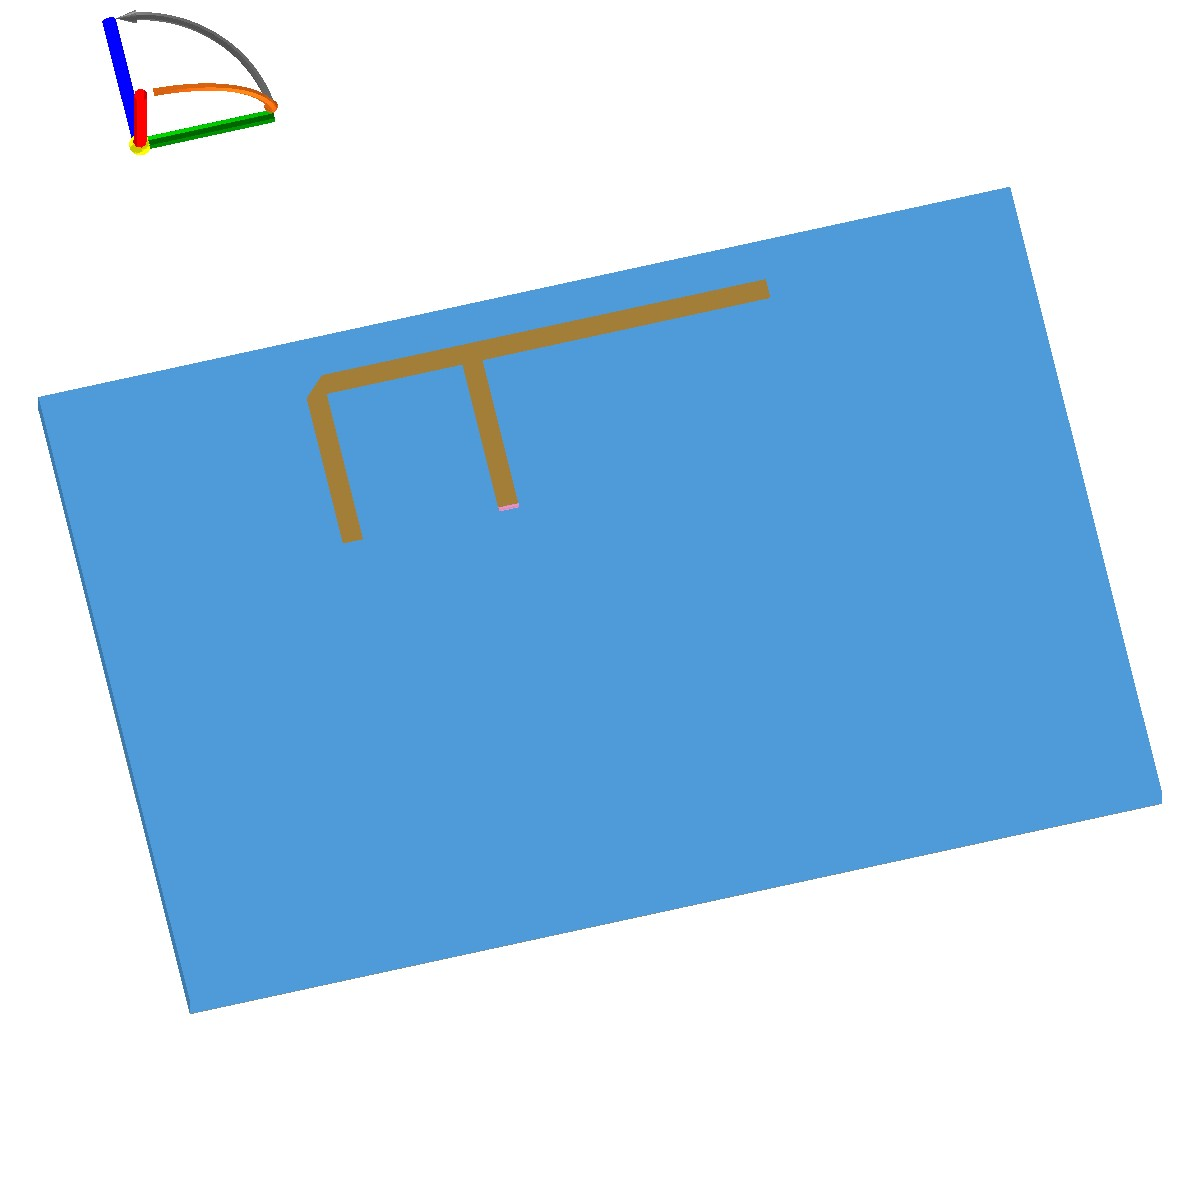
\includegraphics[width=0.5\linewidth]{images/antenna-sketch}
\caption[IFA Layout]{Simulation layout of a single band inverted-F antenna.}
\label{fig:pifa}
\end{figure}

The sensor board looks for three qualities in its antenna, in decreasing importance: cost, range, and compactness. Three antenna configurations were considered for the design. Inverted-F antennas (IFA) are inexpensive and have a reasonable range, but are not as small as chip antennas. Ceramic chip antennas (CCA) are compact, but have poor range, and are expensive. Finally, externally mounted whip antennas have good range, but are also fairly expensive.

\begin{figure}[h]
\centering
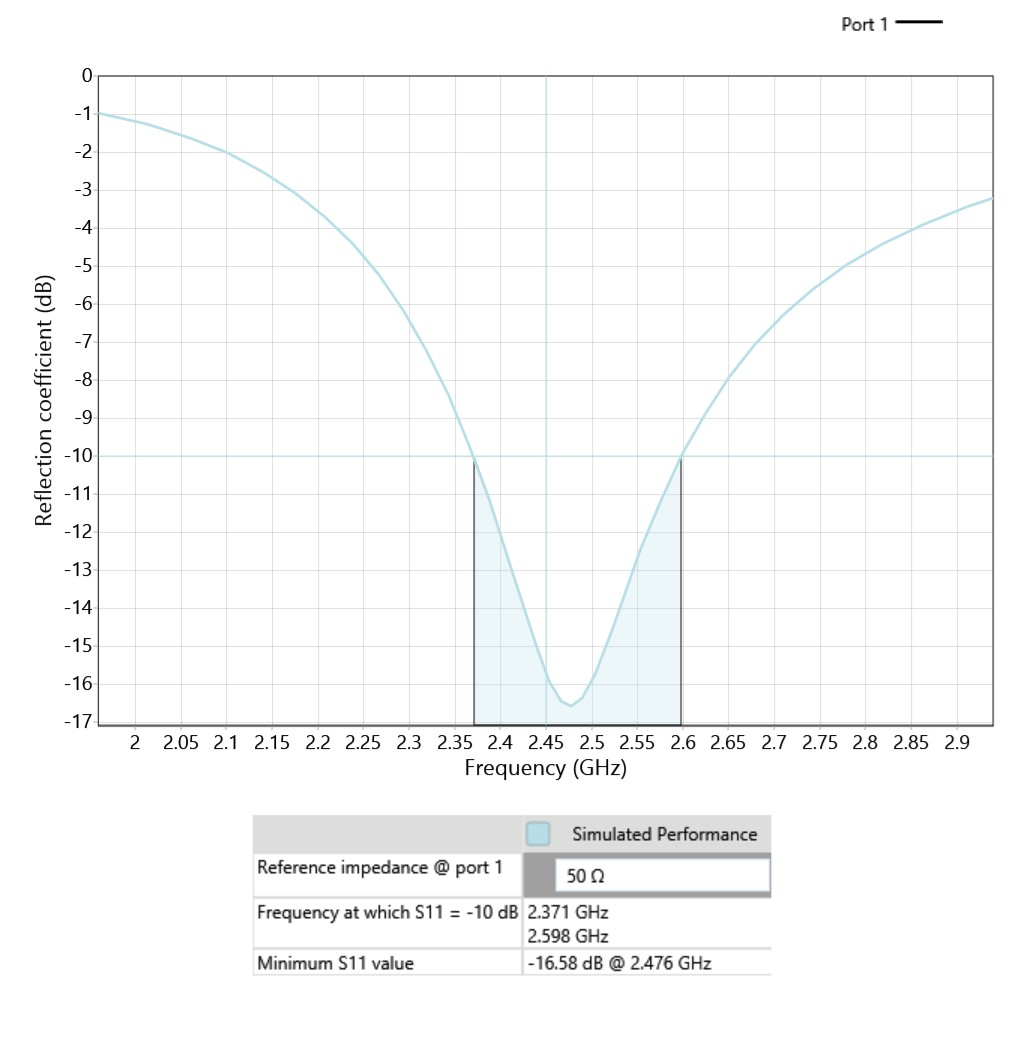
\includegraphics[width=0.5\linewidth]{images/antenna-performance}
\caption[IFA Performance]{Simulated performance of inverted-F antenna}
\label{fig:pifaperf}
\end{figure}

In this design, an IFA was initially selected. An IFA has a simple structure, an omni-directional radiation pattern, and is very low-cost as it is fabricated as part of the PCB. It has an elliptical polarization, allowing it to receive both vertical and horizontally polarized waves\cite{Huynh2000}. This is important in an indoor environment as wireless waves often tend to become depolarized as they reflect off internal surfaces. For all these reasons, inverted-F antennas are extremely common in small electronic devices, and see common application in mobile handsets. One of the additional advantages of the IFA for prototyping is that it can be easily tuned by hand by fabricating the long arm of the F with excess length, and then scraping the excess surface copper until a good impedance match is obtained. An IFA antenna was designed, and the geometry is illustrated in figure \ref{fig:pifa}. The dielectric is standard 2-layer FR4 with a thickness of 1.6mm (63 mil) and 1 oz. copper traces and fills. The antenna  was simulated and found to have good S11 of -13dB in the 2.4 GHz band. 

However, after prototyping, a 50 Ohm microstrip to an edge-launched SMA connector was selected, and the antenna engineering work moved off the PCB. As a development platform, the ability to swap in a highly directional antenna is useful. Directional antennas are an easy way to extend wireless range without consuming more power, and locking the user in to using the provided PCB trace antenna is limiting.

\section{Other Notes}

The system is designed to run autonomously with little interaction by the user. Accordingly, there is only one reset button on the board, along with three status LEDs. If additional physical user interaction is required, they can be added to the 0.1" header. 

In order to facilitate easy development, an FTDI dual serial to USB chip is included on the board's footprint. One port connects to the CC3200 UART, and another to the CC3200 JTAG pins. This simplifies the development process as a JTAG probe set is no longer needed for in-circuit debugging and firmware flashing. The FTDI chip runs completely from USB power, so it consumes no energy in the battery-powered use case. The previous generation MSP430-based nodes often had the problem that the JTAG circuit probes often be unavailable, so this was a key upgrade.

The CC3200 SoC is over-specified for the base use-case, and contains spare computational and memory capacity. The internal ARM-M4 micro-controller runs at 80 MHz from a pair of external 32.768 kHz and 40 MHz crystal oscillators. The model specified in this design contains 128 kB of RAM and is run from an 8 MB serial flash module accessed over the SPI bus. As the current firmware load consumes around 40 kilobytes of RAM during regular operation, expanded functionality can easily be programmed in the future.


